\chapter{Análisis \label{sec:analisis}}
En este apartado se procederá a realizar un estudio de las funciones que deberá cumplir la arquitectura \textit{big data} implementada finalmente. Para ello, en este apartado se incluye la colección de requisitos del sistema definidos antes de comenzar el desarrollo del mismo.

Estos requisitos junto con el análisis de realizado de las tecnologías que se van a emplear, el estudio del problema propuesto por la organización del concurso y de los datos que se introducirán en el sistema, que serán las trazas de los viajes de los taxis de Nueva York, establecerán las guías para el diseño e implementación de la arquitectura \textit{big data} que se va a desarrollar y, tras la finalización de este proceso, serán utilizados para la comprobación de la verificación de completitud de los objetivos de este proyecto.

Al final de este apartado se incluirá una matriz de trazabilidad para trazar la relación entre los requisitos de usuario y los de software.

\section{Requisitos de usuario}
Para este proyecto, debido a la falta de un cliente, los requisitos de usuario han sido establecidos en conjunto por el autor y el tutor del trabajo. En estos se recogen las claves que deberá cumplir la arquitectura para lograr los objetivos establecidos y se dividen en dos conjuntos claramente diferenciados:

\begin{itemize}
\item \textbf{Requisitos de capacidad:} Que son aquellas funciones y objetivos que el sistema deberá cumplir para satisfacer al usuario.
\item \textbf{Requisitos de restricción:} Que establecen los límites que la arquitectura debe respetar a la hora de desarrollar el proyecto.
\end{itemize}

La nomenclatura que se utilizará para definir estos requisitos será la siguiente:

\begin{itemize}
\item \textbf{RU:} Que identificará al requisito como de usuario.
\item \textbf{C o R:} Que establecerá si el requisito es de capacidad (C) o de restricción (R).
\item \textbf{XX:} Donde XX es un número y que, con el conjunto de requisitos, formará una secuencia numérica que irá de 00 a 99. Este indica el número del requisito y la secuencia será independiente de cada tipo de requisito.
\end{itemize}

Por tanto, un requisito de usuario será identificado mediante la siguiente estructura RU-(C, R)-XX. La descripción de estos requisitos contará con los siguientes campos:


\begin{itemize}
\item \textbf{Identificador:} Identificación del requisito mediante la nomenclatura explicada anteriormente.
\item \textbf{Fuente:} Creador del requisito de usuario. Este podrá ser el autor o el tutor del proyecto.
\item \textbf{Necesidad:} Nivel de importancia respecto al cumplimiento del requisito:
\begin{itemize}
\item \textit{Fundamental:} Requisito de obligatorio cumplimiento en la implementación realizada.
\item \textit{Recomendable:} Requisito que es deseable que cumpla el sistema.
\item \textit{Prescindible:} Requisito que no supone ningún problema en caso de no ser implementado.
\end{itemize}
\item \textbf{Prioridad:} Establece la importancia del requisito respecto a la planificación de su implementación. Podrá ser \textit{alta}, \textit{media} o \textit{baja}.
\item \textbf{Descripción:} Texto que establecerá y describirá la función o restricción que deberá cumplir el sistema.
\end{itemize}

\begin{table}[htp!]
\centering
\caption{Requisito de usuario RU-C-01}
\label{ru1}
\begin{tabular}{|c|l|c|l|}
\hline
\textbf{IDENTIFICADOR} & \multicolumn{3}{l|}{RU-C-01}            \\ \hline
\textbf{FUENTE}        & \multicolumn{3}{l|}{Tutor}              \\ \hline
\textbf{NECESIDAD}     & Fundamental & \textbf{PRIORIDAD} & Alta \\ \hline
\multicolumn{4}{|c|}{\textbf{DESCRIPCIÓN}}                       \\ \hline
\multicolumn{4}{|l|}{\begin{tabular}[c]{@{}l@{}}Los ficheros a emplear por el sistema serán\\ las trazas de los viajes de taxis de la ciudad de Nueva York\\ proporcionados por la competición\end{tabular}} \\ \hline
\end{tabular}
\end{table}

\begin{table}[htp!]
\centering
\caption{Requisito de usuario RU-C-02}
\label{ru2}
\begin{tabular}{|c|l|c|l|}
\hline
\textbf{IDENTIFICADOR} & \multicolumn{3}{l|}{RU-C-02}            \\ \hline
\textbf{FUENTE}        & \multicolumn{3}{l|}{Tutor}              \\ \hline
\textbf{NECESIDAD}     & Fundamental & \textbf{PRIORIDAD} & Alta \\ \hline
\multicolumn{4}{|c|}{\textbf{DESCRIPCIÓN}}                       \\ \hline
\multicolumn{4}{|l|}{El sistema debe ser capaz de procesar los datos de forma masiva}\\ \hline
\end{tabular}
\end{table}

\begin{table}[htp!]
\centering
\caption{Requisito de usuario RU-C-03}
\label{ru3}
\begin{tabular}{|c|l|c|l|}
\hline
\textbf{IDENTIFICADOR} & \multicolumn{3}{l|}{RU-C-03}            \\ \hline
\textbf{FUENTE}        & \multicolumn{3}{l|}{Tutor}              \\ \hline
\textbf{NECESIDAD}     & Fundamental & \textbf{PRIORIDAD} & Alta \\ \hline
\multicolumn{4}{|c|}{\textbf{DESCRIPCIÓN}}                       \\ \hline
\multicolumn{4}{|l|}{\begin{tabular}[c]{@{}l@{}}El sistema debe de ser capaz de adaptar los datos al problema\\ y realizar la eliminación de los registros inválidos\end{tabular}} \\ \hline
\end{tabular}
\end{table}

\begin{table}[htp!]
\centering
\caption{Requisito de usuario RU-C-04}
\label{ru4}
\begin{tabular}{|c|l|c|l|}
\hline
\textbf{IDENTIFICADOR} & \multicolumn{3}{l|}{RU-C-04}            \\ \hline
\textbf{FUENTE}        & \multicolumn{3}{l|}{Tutor}              \\ \hline
\textbf{NECESIDAD}     & Fundamental & \textbf{PRIORIDAD} & Alta \\ \hline
\multicolumn{4}{|c|}{\textbf{DESCRIPCIÓN}}                       \\ \hline
\multicolumn{4}{|l|}{\begin{tabular}[c]{@{}l@{}}El sistema debe de ser capaz de analizar los datos\\ y responder a las consultas planteadas en el problema\end{tabular}} \\ \hline
\end{tabular}
\end{table}

\begin{table}[htp!]
\centering
\caption{Requisito de usuario RU-C-05}
\label{ru5}
\begin{tabular}{|c|l|c|l|}
\hline
\textbf{IDENTIFICADOR} & \multicolumn{3}{l|}{RU-C-05}            \\ \hline
\textbf{FUENTE}        & \multicolumn{3}{l|}{Tutor}              \\ \hline
\textbf{NECESIDAD}     & Fundamental & \textbf{PRIORIDAD} & Alta \\ \hline
\multicolumn{4}{|c|}{\textbf{DESCRIPCIÓN}}                       \\ \hline
\multicolumn{4}{|l|}{El sistema debe poder implementarse en diversos entornos y condiciones}\\ \hline
\end{tabular}
\end{table}

\begin{table}[htp!]
\centering
\caption{Requisito de usuario RU-C-06}
\label{ru6}
\begin{tabular}{|c|l|c|l|}
\hline
\textbf{IDENTIFICADOR} & \multicolumn{3}{l|}{RU-C-06}            \\ \hline
\textbf{FUENTE}        & \multicolumn{3}{l|}{Tutor}              \\ \hline
\textbf{NECESIDAD}     & Fundamental & \textbf{PRIORIDAD} & Media \\ \hline
\multicolumn{4}{|c|}{\textbf{DESCRIPCIÓN}}                       \\ \hline
\multicolumn{4}{|l|}{Se debe comparar el rendimiento de las diferentes configuraciones implementadas}\\ \hline
\end{tabular}
\end{table}

\begin{table}[htp!]
\centering
\caption{Requisito de usuario RU-C-07}
\label{ru7}
\begin{tabular}{|c|l|c|l|}
\hline
\textbf{IDENTIFICADOR} & \multicolumn{3}{l|}{RU-C-07}            \\ \hline
\textbf{FUENTE}        & \multicolumn{3}{l|}{Tutor}              \\ \hline
\textbf{NECESIDAD}     & Fundamental & \textbf{PRIORIDAD} & Media \\ \hline
\multicolumn{4}{|c|}{\textbf{DESCRIPCIÓN}}                       \\ \hline
\multicolumn{4}{|l|}{\begin{tabular}[c]{@{}l@{}}Se deben comparar el rendimiento del sistema con\\ diferentes tamaños del fichero de datos\end{tabular}} \\ \hline
\end{tabular}
\end{table}

\begin{table}[htp!]
\centering
\caption{Requisito de usuario RU-C-08}
\label{ru8}
\begin{tabular}{|c|l|c|l|}
\hline
\textbf{IDENTIFICADOR} & \multicolumn{3}{l|}{RU-C-08}            \\ \hline
\textbf{FUENTE}        & \multicolumn{3}{l|}{Autor del TFG}      \\ \hline
\textbf{NECESIDAD}     & Importante & \textbf{PRIORIDAD} & Normal\\ \hline
\multicolumn{4}{|c|}{\textbf{DESCRIPCIÓN}}                       \\ \hline
\multicolumn{4}{|l|}{\begin{tabular}[c]{@{}l@{}}No se define ninguna interfaz de usuario, el sistema\\  se ejecutará mediante la línea de comandos de Linux\end{tabular}} \\ \hline
\end{tabular}
\end{table}

\begin{table}[htp!]
\centering
\caption{Requisito de usuario RU-C-09}
\label{ru9}
\begin{tabular}{|c|l|c|l|}
\hline
\textbf{IDENTIFICADOR} & \multicolumn{3}{l|}{RU-C-09}            \\ \hline
\textbf{FUENTE}        & \multicolumn{3}{l|}{Autor del TFG}      \\ \hline
\textbf{NECESIDAD}     & Fundamental & \textbf{PRIORIDAD} & Alta \\ \hline
\multicolumn{4}{|c|}{\textbf{DESCRIPCIÓN}}                       \\ \hline
\multicolumn{4}{|l|}{\begin{tabular}[c]{@{}l@{}}Se debe documentar todo el estudio previo, el desarollo del\\ sistema y el análisis de los resultados obtenidos\end{tabular}} \\ \hline
\end{tabular}
\end{table}


\begin{table}[htp!]
\centering
\caption{Requisito de usuario RU-R-01}
\label{rur1}
\begin{tabular}{|c|l|c|l|}
\hline
\textbf{IDENTIFICADOR} & \multicolumn{3}{l|}{RU-R-01}            \\ \hline
\textbf{FUENTE}        & \multicolumn{3}{l|}{Tutor}              \\ \hline
\textbf{NECESIDAD}     & Fundamental & \textbf{PRIORIDAD} & Alta \\ \hline
\multicolumn{4}{|c|}{\textbf{DESCRIPCIÓN}}                       \\ \hline
\multicolumn{4}{|l|}{Se deberá usar \textit{Apache Spark} como librería principal de la arquitectura}\\ \hline
\end{tabular}
\end{table}

\begin{table}[htp!]
\centering
\caption{Requisito de usuario RU-R-02}
\label{rur2}
\begin{tabular}{|c|l|c|l|}
\hline
\textbf{IDENTIFICADOR} & \multicolumn{3}{l|}{RU-R-02}            \\ \hline
\textbf{FUENTE}        & \multicolumn{3}{l|}{Tutor}              \\ \hline
\textbf{NECESIDAD}     & Fundamental & \textbf{PRIORIDAD} & Alta \\ \hline
\multicolumn{4}{|c|}{\textbf{DESCRIPCIÓN}}                       \\ \hline
\multicolumn{4}{|l|}{Se deberá utilizar Python para realizar el desarrollo del sistema}\\ \hline
\end{tabular}
\end{table}

\section{Requisitos de software}
En este apartado, teniendo como base los requisitos de usuario enumerados anteriormente y con el conocimiento adquirido tras el análisis del problema planteado y del fichero de las trazas de los viajes de taxi, se definirán los requisitos de software. La nomenclatura utilizada para estos requisitos será ```RS-(F, NF-R, NF-D)-XX'' donde:

\begin{itemize}
\item \textbf{RS:} Que identificará al requisito como de usuario.
\item \textbf{F, NF-R o NF-D:} Que establecerá si el requisito es funcional (F) o no funcional, ya sea de restricción (R) o de documentación (D).
\item \textbf{XX:} Donde XX es un número y que, con el conjunto de requisitos, formará una secuencia numérica que irá de 00 a 99. Este indica el número del requisito y la secuencia será independiente de cada tipo de requisito.
\end{itemize}

Por tanto, un requisito de usuario será identificado mediante la siguiente estructura RU-(C, R)-XX. La descripción de estos requisitos contará con los siguientes campos:

\begin{itemize}
\item \textbf{RS:} Que identificará al requisito como de usuario.
\item \textbf{C o R:} Que establecerá si el requisito es de capacidad (C) o de restricción (R).
\item \textbf{XX:} Donde XX es un número y que, con el conjunto de requisitos, formará una secuencia numérica que irá de 00 a 99. Este indica el número del requisito y la secuencia será independiente de cada tipo de usuario.
\end{itemize}

\begin{itemize}
\item \textbf{Identificador:} Identificación del requisito mediante la nomenclatura explicada anteriormente.
\item \textbf{Fuente:} Que indica el requisito de usuario en el que se basa.
\item \textbf{Necesidad:} Se mantiene de la misma forma que en los requisitos de usuario.
\item \textbf{Prioridad:} Se mantiene de la misma forma que en los requisitos de usuario.
\item \textbf{Descripción:} Texto que establecerá y describirá el objetivo del requisito.
\end{itemize}

\begin{table}[htp!]
\centering
\caption{Requisito de software RS-F-01}
\label{rs1}
\begin{tabular}{|c|l|c|l|}
\hline
\textbf{IDENTIFICADOR}                                                                                       & \multicolumn{3}{l|}{RS-F-01}                                                                                                                                                                                                                                                                     \\ \hline
\textbf{FUENTE}                                                                                              & \multicolumn{3}{l|}{RU-C-01}                                                                                                                                                                                                                                                                     \\ \hline
\textbf{NECESIDAD}                                                                                           & Fundamental                                                                                       & PRIORIDAD                                                                                       & Alta                                                                                       \\ \hline
\multicolumn{4}{|c|}{\textbf{DESCRIPCIÓN}}                                                                                                                                                                                                                                                                                                                                                                      \\ \hline
\multicolumn{4}{|l|}{\begin{tabular}[c]{@{}l@{}}El fichero de datos que utilice el sistema será\\ el obtenido de la página del concurso \cite{grandChallenge},\\ que contendrá las trazas de los viajes de taxi de\\ la ciudad de Nueva York durante el año 2013, \\ siendo este fichero un \gls{CSV} de 33 GB.\\ Cada línea de este fichero representará un viaje y\\ cada registro contendrá 17 atributos\end{tabular}} \\ \hline
\end{tabular}
\end{table}

\begin{table}[htp!]
\centering
\caption{Requisito de software RS-F-02}
\label{rs2}
\begin{tabular}{|c|l|c|l|}
\hline
\textbf{IDENTIFICADOR}                                          & \multicolumn{3}{l|}{RS-F-02}                                                                                                                           \\ \hline
\textbf{FUENTE}                                                 & \multicolumn{3}{l|}{RU-C-02}                                                                                                                           \\ \hline
\textbf{NECESIDAD}                                              & Fundamental                                         & PRIORIDAD                                         & Alta                                         \\ \hline
\multicolumn{4}{|c|}{\textbf{DESCRIPCIÓN}}                                                                                                                                                                               \\ \hline
\multicolumn{4}{|l|}{\begin{tabular}[c]{@{}l@{}}El sistema debe ser capaz de procesar y realizar las \\ tareas que se ejecuten sobre los ficheros disponibles\\ sin problemas ni excepciones de ejecución.\end{tabular}} \\ \hline
\end{tabular}
\end{table}

\begin{table}[htp!]
\centering
\caption{Requisito de software RS-F-03}
\label{rs3}
\begin{tabular}{|c|l|c|l|}
\hline
\textbf{IDENTIFICADOR}                                   & \multicolumn{3}{l|}{RS-F-03}                                                                                                      \\ \hline
\textbf{FUENTE}                                          & \multicolumn{3}{l|}{RU-C-03}                                                                                                      \\ \hline
\textbf{NECESIDAD}                                       & Fundamental                                  & PRIORIDAD                                  & Alta                                  \\ \hline
\multicolumn{4}{|c|}{\textbf{DESCRIPCIÓN}}                                                                                                                                                   \\ \hline
\multicolumn{4}{|l|}{\begin{tabular}[c]{@{}l@{}}El sistema debe ser capaz de detectar los registros con errores y\\ de eliminarlos del fichero de datos para su posterior uso\end{tabular}} \\ \hline
\end{tabular}
\end{table}

\begin{table}[htp!]
\centering
\caption{Requisito de software RS-F-04}
\label{rs4}
\begin{tabular}{|c|l|c|l|}
\hline
\textbf{IDENTIFICADOR}                                          & \multicolumn{3}{l|}{RS-F-04}                                                                                                                              \\ \hline
\textbf{FUENTE}                                                 & \multicolumn{3}{l|}{RU-C-03}                                                                                                                              \\ \hline
\textbf{NECESIDAD}                                              & Fundamental                                          & PRIORIDAD                                          & Alta                                          \\ \hline
\multicolumn{4}{|c|}{\textbf{DESCRIPCIÓN}}                                                                                                                                                                                  \\ \hline
\multicolumn{4}{|l|}{\begin{tabular}[c]{@{}l@{}}El sistema debe ser capaz de transformar los atributos de  los\\ registros para adaptarlos a los requisitos del problema y guardarlos\\ para su posterior uso\end{tabular}} \\ \hline
\end{tabular}
\end{table}

\begin{table}[htp!]
\centering
\caption{Requisito de software RS-F-05}
\label{rs5}
\begin{tabular}{|c|l|c|l|}
\hline
\textbf{IDENTIFICADOR}                                 & \multicolumn{3}{l|}{RS-F-05}                                                                                                 \\ \hline
\textbf{FUENTE}                                        & \multicolumn{3}{l|}{RU-C-04}                                                                                                 \\ \hline
\textbf{NECESIDAD}                                     & Fundamental                                 & PRIORIDAD                                & Alta                                \\ \hline
\multicolumn{4}{|c|}{\textbf{DESCRIPCIÓN}}                                                                                                                                            \\ \hline
\multicolumn{4}{|l|}{\begin{tabular}[c]{@{}l@{}}El sistema debe ser capaz de analizar los datos procesados \\ anteriormente para calcular las diez rutas más frecuentes\end{tabular}} \\ \hline
\end{tabular}
\end{table}

\begin{table}[htp!]
\centering
\caption{Requisito de software RS-F-06}
\label{rs6}
\begin{tabular}{|c|l|c|l|}
\hline
\textbf{IDENTIFICADOR}                                       & \multicolumn{3}{l|}{RS-F-06}                                                                                                                     \\ \hline
\textbf{FUENTE}                                              & \multicolumn{3}{l|}{RU-C-04}                                                                                                                     \\ \hline
\textbf{NECESIDAD}                                           & Fundamental                                       & PRIORIDAD                                       & Alta                                       \\ \hline
\multicolumn{4}{|c|}{\textbf{DESCRIPCIÓN}}                                                                                                                                                                      \\ \hline
\multicolumn{4}{|l|}{\begin{tabular}[c]{@{}l@{}}El sistema debe ser capaz de analizar los datos procesados \\ anteriormente para calcular las diez zonas que más beneficios\\ reporten al taxista\end{tabular}} \\ \hline
\end{tabular}
\end{table}

\begin{table}[htp!]
\centering
\caption{Requisito de software RS-F-07}
\label{rs7}
\begin{tabular}{|c|l|c|l|}
\hline
\textbf{IDENTIFICADOR}                            & \multicolumn{3}{l|}{RS-F-07}                                                                                 \\ \hline
\textbf{FUENTE}                                   & \multicolumn{3}{l|}{RU-C-05}                                                                                 \\ \hline
\textbf{NECESIDAD}                                & Fundamental                           & PRIORIDAD                           & Alta                           \\ \hline
\multicolumn{4}{|c|}{\textbf{DESCRIPCIÓN}}                                                                                                                       \\ \hline
\multicolumn{4}{|l|}{\begin{tabular}[c]{@{}l@{}}El sistema debe ser implementado en el entorno doméstico\\ tanto en el modo local como distribuido\end{tabular}} \\ \hline
\end{tabular}
\end{table}

\begin{table}[htp!]
\centering
\caption{Requisito de software RS-F-08}
\label{rs8}
\begin{tabular}{|c|l|c|l|}
\hline
\textbf{IDENTIFICADOR}                             & \multicolumn{3}{l|}{RS-F-07}                                                                                    \\ \hline
\textbf{FUENTE}                                    & \multicolumn{3}{l|}{RU-C-05}                                                                                    \\ \hline
\textbf{NECESIDAD}                                 & Fundamental                            & PRIORIDAD                            & Alta                            \\ \hline
\multicolumn{4}{|c|}{\textbf{DESCRIPCIÓN}}                                                                                                                           \\ \hline
\multicolumn{4}{|l|}{\begin{tabular}[c]{@{}l@{}}El sistema debe ser implementado en el entorno universitario\\ tanto en el modo local como distribuido\end{tabular}} \\ \hline
\end{tabular}
\end{table}

\begin{table}[htp!]
\centering
\caption{Requisito de software RS-F-09}
\label{rs9}
\begin{tabular}{|c|l|c|l|}
\hline
\textbf{IDENTIFICADOR}                                           & \multicolumn{3}{l|}{RS-F-09}                                                                                                                               \\ \hline
\textbf{FUENTE}                                                  & \multicolumn{3}{l|}{RU-C-06}                                                                                                                               \\ \hline
\textbf{NECESIDAD}                                               & Fundamental                                           & PRIORIDAD                                          & Media                                          \\ \hline
\multicolumn{4}{|c|}{\textbf{DESCRIPCIÓN}}                                                                                                                                                                                    \\ \hline
\multicolumn{4}{|l|}{\begin{tabular}[c]{@{}l@{}}Se compararán los resultados de rendimiento de los diferentes\\ modos implementados, local o distribuido, y los diferentes \\ entornos, doméstico y universitario\end{tabular}} \\ \hline
\end{tabular}
\end{table}

\begin{table}[htp!]
\centering
\caption{Requisito de software RS-F-10}
\label{rs10}
\begin{tabular}{|c|l|c|l|}
\hline
\textbf{IDENTIFICADOR}                                      & \multicolumn{3}{l|}{RS-F-10}                                                                                                                   \\ \hline
\textbf{FUENTE}                                             & \multicolumn{3}{l|}{RU-C-07}                                                                                                                   \\ \hline
\textbf{NECESIDAD}                                          & Fundamental                                      & PRIORIDAD                                      & Media                                      \\ \hline
\multicolumn{4}{|c|}{\textbf{DESCRIPCIÓN}}                                                                                                                                                                   \\ \hline
\multicolumn{4}{|l|}{\begin{tabular}[c]{@{}l@{}}Se realizarán diversos ficheros de datos a partir del\\ original, de menor tamaño, para comparar los resultados\\ de procesamiento entre ellos\end{tabular}} \\ \hline
\end{tabular}
\end{table}

\begin{table}[htp!]
\centering
\caption{Requisito de software RS-F-011}
\label{rs11}
\begin{tabular}{|c|l|c|l|}
\hline
\textbf{IDENTIFICADOR}                                              & \multicolumn{3}{l|}{RS-F-11}                                                                                                                                        \\ \hline
\textbf{FUENTE}                                                     & \multicolumn{3}{l|}{RU-C-08}                                                                                                                                        \\ \hline
\textbf{NECESIDAD}                                                  & Fundamental                                             & PRIORIDAD                                             & Media                                             \\ \hline
\multicolumn{4}{|c|}{\textbf{DESCRIPCIÓN}}                                                                                                                                                                                                \\ \hline
\multicolumn{4}{|l|}{\begin{tabular}[c]{@{}l@{}}La ejecución de las diferentes funciones del sistema\\ se realizará a través de la de línea de comandos de Linux,\\ mediante la introducción de la función y sus argumentos\end{tabular}} \\ \hline
\end{tabular}
\end{table}

\begin{table}[htp!]
\centering
\caption{Requisito de software RS-NF-D-01}
\label{rsnf1}
\begin{tabular}{|c|l|c|l|}
\hline
\textbf{IDENTIFICADOR}                                                                                & \multicolumn{3}{l|}{RS-NF-D-01}                                                                                                                                                                                                                                              \\ \hline
\textbf{FUENTE}                                                                                       & \multicolumn{3}{l|}{RU-C-09}                                                                                                                                                                                                                                                 \\ \hline
\textbf{NECESIDAD}                                                                                    & Fundamental                                                                                 & PRIORIDAD                                                                                & Alta                                                                                \\ \hline
\multicolumn{4}{|c|}{\textbf{DESCRIPCIÓN}}                                                                                                                                                                                                                                                                                                                                           \\ \hline
\multicolumn{4}{|l|}{\begin{tabular}[c]{@{}l@{}}Se realizará una memoria del trabajo realizado, donde\\ se incluirá el estado del arte y el análisis de la situación\\ de las tecnologías utilizadas, así como, un análisis de los\\ pasos seguidos durante el desarrollo de la arquitectura, \\ incluyendo el diseño, la implementación y los resultados\\ obtenidos.\end{tabular}} \\ \hline
\end{tabular}
\end{table}

\begin{table}[htp!]
\centering
\caption{Requisito de software RS-NF-R-01}
\label{rsfn2}
\begin{tabular}{|c|l|c|l|}
\hline
\textbf{IDENTIFICADOR}                                                   & \multicolumn{3}{l|}{RS-NF-R-01}                                                                                                                                                       \\ \hline
\textbf{FUENTE}                                                          & \multicolumn{3}{l|}{RU-R-01}                                                                                                                                                          \\ \hline
\textbf{NECESIDAD}                                                       & Fundamental                                                    & PRIORIDAD                                                   & Alta                                                   \\ \hline
\multicolumn{4}{|c|}{\textbf{DESCRIPCIÓN}}                                                                                                                                                                                                                       \\ \hline
\multicolumn{4}{|l|}{\begin{tabular}[c]{@{}l@{}}Se utilizará \textit{Apache Spark} como librería principal del \\ proyecto, siendo utilizada para gestionar los procesos\\ llevados a cabo por el sistema, tanto en el modo local\\ como en el distribuido.\end{tabular}} \\ \hline
\end{tabular}
\end{table}

\begin{table}[htp!]
\centering
\caption{Requisito de software RS-NF-R-02}
\label{rsnf3}
\begin{tabular}{|c|l|c|l|}
\hline
\textbf{IDENTIFICADOR}                                      & \multicolumn{3}{l|}{RS-NF-R-02}                                                                                                              \\ \hline
\textbf{FUENTE}                                             & \multicolumn{3}{l|}{RU-R-02}                                                                                                                 \\ \hline
\textbf{NECESIDAD}                                          & Fundamental                                       & PRIORIDAD                                     & Alta                                     \\ \hline
\multicolumn{4}{|c|}{\textbf{DESCRIPCIÓN}}                                                                                                                                                                 \\ \hline
\multicolumn{4}{|l|}{\begin{tabular}[c]{@{}l@{}}Se utilizará Python como lenguaje de programación para\\ el desarrollo del sistema, utilizando la API de \textit{Apache Spark},\\ pyspark, para ello.\end{tabular}} \\ \hline
\end{tabular}
\end{table}

\section{Matriz de trazabilidad}
\begin{figure}[htp!]
\centering
\caption{Matriz de trazabilidad de los requisitos}
\label{tab:matrizReq}
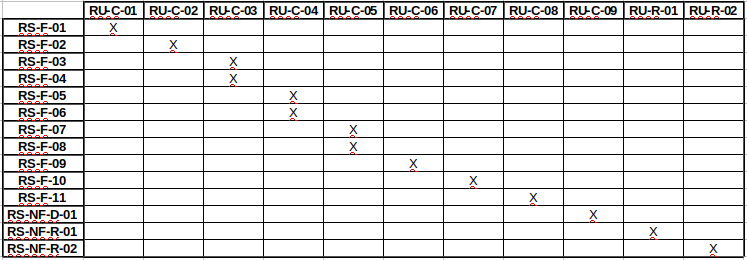
\includegraphics[scale=0.6]{graphics/matriz}
\end{figure}